\documentclass[12pt, oneside]{article} 
\usepackage{amsmath, amsthm, amssymb, calrsfs, wasysym, verbatim, bbm, color, graphics, geometry, enumitem, array, multirow, hyperref, tabulary, xcolor}

\usepackage{amsmath,amssymb,mathtools} % do fancy math
\usepackage{graphicx} % import images
\usepackage{xcolor}
\usepackage{tikz} % draw images with latex
\usepackage{listings} % for code 
\usepackage{enumitem, bm, bbm}
% \usepackage{amsfonts}
\usepackage[onehalfspacing]{setspace}

\usepackage{subcaption}




\setlength{\parindent}{0in} % set paragraph indent
\everymath{\displaystyle}
\setlist{noitemsep}


\geometry{top=1in, bottom=1in, left=1in, right=1in}
\setlist{noitemsep}
%\setcounter{secnumdepth}{0} % comment this out for section numbering
\everymath{\displaystyle}

\geometry{top=1in, bottom=1in, left=1in, right=1in}
\setlist{noitemsep}
%\setcounter{secnumdepth}{0} % comment this out for section numbering
\everymath{\displaystyle}

% Math symbols
\newcommand*{\T}{^{\top}}
\renewcommand*{\i}{\leftarrow}
\newcommand*{\isim}{\overset{\text{ind}}{\sim}}
\newcommand*{\iid}{\overset{\text{i.i.d.}}{\sim}}
\newcommand*{\deq}{\overset{\text{d}}{=}}
% Sets (natural numbers etc)
\newcommand*{\IN}{\mathbb{N}} 
\newcommand*{\IZ}{\mathbb{Z}}
\newcommand*{\IQ}{\mathbb{Q}}
\newcommand*{\IR}{\mathbb{R}}
\newcommand*{\IC}{\mathbb{C}}
% Distributions, processes
\newcommand*{\Geo}{\operatorname{Geo}}
\newcommand*{\Exp}{\operatorname{Exp}}
\newcommand*{\Poi}{\operatorname{Poi}}
\newcommand*{\NVM}{\operatorname{NVM}}
\newcommand*{\Par}{\operatorname{Par}}
\newcommand*{\IG}{\operatorname{IG}}
\newcommand*{\LN}{\operatorname{LN}}
\newcommand*{\Cauchy}{\operatorname{Cauchy}}
\newcommand*{\Log}{\operatorname{Log}}
\newcommand*{\U}{\operatorname{U}} % uniform distribution
\newcommand*{\B}{\operatorname{B}}
\newcommand*{\Bin}{\operatorname{Bin}}
\newcommand*{\Bern}{\operatorname{Bern}}
\newcommand*{\Beta}{\operatorname{Beta}}
\newcommand*{\NB}{\operatorname{NB}}
\newcommand*{\N}{\operatorname{N}}
% Operators, functions
\newcommand*{\I}{\mathbbm{1}} % indicator 
\newcommand*{\rd}{\mathrm{d}} % differential in integrals 
\renewcommand*{\mod}{\operatorname{mod}}
\newcommand*{\arginf}{\operatorname*{arginf}}
\newcommand*{\argsup}{\operatorname*{argsup}}
\newcommand*{\ran}{\operatorname{ran}}
\newcommand*{\rank}{\operatorname{rank}}
\newcommand*{\sign}{\operatorname{sign}}
\newcommand*{\round}{\operatorname{round}}
\renewcommand*{\L}{\mathcal{L}}
\renewcommand*{\Re}{\operatorname{Re}}
\renewcommand*{\Im}{\operatorname{Im}}
\newcommand*{\Li}{\operatorname*{Li}}
\renewcommand*{\P}{\mathbb{P}} % probability
\newcommand*{\E}{\mathbb{E}} % expected value 
\newcommand*{\med}{\operatorname{med}}
\newcommand*{\Var}{\operatorname{Var}}
\newcommand*{\Cov}{\operatorname{Cov}}
\newcommand*{\Cor}{\operatorname{Cor}}
\newcommand*{\MSE}{\operatorname{MSE}}
\newcommand*{\SE}{\operatorname{SE}}

% Variables
\newcommand*{\R}{\textsf{R}}
\newcommand*{\eps}{\varepsilon}
\renewcommand*{\th}{\bm{\theta}}
\newcommand*{\ba}{\bm{a}}
\newcommand*{\bnu}{\bm{\nu}}
\newcommand*{\bb}{\bm{b}}
\newcommand*{\be}{\bm{e}}
\newcommand*{\blambda}{\bm{\lambda}}
\newcommand*{\bzero}{\bm{0}}
\newcommand*{\bone}{\bm{1}}
\newcommand*{\bt}{\bm{t}}
\newcommand*{\bx}{\bm{x}}
\newcommand*{\by}{\bm{y}}
\newcommand*{\bz}{\bm{z}}
\newcommand*{\bu}{\bm{u}}
\newcommand*{\bU}{\bm{U}}
\newcommand*{\bv}{\bm{v}}
\newcommand*{\bw}{\bm{w}}
\newcommand*{\btheta}{\bm{\theta}}
\newcommand*{\bS}{\bm{S}}
\newcommand*{\bT}{\bm{T}}
\newcommand*{\bZ}{\bm{Z}}
\newcommand*{\bY}{\bm{Y}}
\newcommand*{\bX}{\bm{X}}
\newcommand*{\bmu}{\bm{\mu}}
% Estimators 
\newcommand*{\hgamma}{\widehat{\gamma}}
\newcommand*{\halpha}{\widehat{\alpha}}
\newcommand*{\hbeta}{\widehat{\beta}}
\newcommand*{\hlambda}{\widehat{\lambda}}
\newcommand*{\hmu}{\widehat{\mu}}
\newcommand*{\hp}{\widehat{p}}
\newcommand*{\hpi}{\widehat{\pi}}
\newcommand*{\hr}{\widehat{r}}
\newcommand*{\htau}{\widehat{\tau}}
\newcommand*{\htheta}{\widehat{\theta}}
\newcommand*{\hsigma}{\widehat{\sigma}}
\newcommand*{\tbeta}{\widetilde{\beta}}
\newcommand*{\tgamma}{\widetilde{\gamma}}
\newcommand*{\tlambda}{\widetilde{\lambda}}
\newcommand*{\tmu}{\widetilde{\mu}}
\newcommand*{\tpi}{\widetilde{\pi}}
\newcommand*{\tsigma}{\widetilde{\sigma}}
\newcommand*{\ttau}{\widetilde{\tau}}
\newcommand*{\barx}{\overline x}
\newcommand*{\barY}{\overline Y}
\newcommand*{\bary}{\overline y}
\DeclareMathOperator*{\argmax}{argmax} % thin space, limits underneath in displays
\usepackage{listings}
\lstset{ 
  language=R,               
  basicstyle=\small\ttfamily,   
  numbers=left,                  
  numberstyle=\tiny\color{gray},  
  stepnumber=1,                   
  showspaces=false,               
  showstringspaces=false,         
  showtabs=false,                  
  tabsize=4,                      
  captionpos=b,                   
  breaklines=true,               
  breakatwhitespace=false,        
  keywordstyle=\color{blue},    
  commentstyle=\color{purple}, 
  stringstyle=\color{Green}     
} 
\title{STAT 441}
\date{W2021}


\linespread{1.3}
\begin{document}

\maketitle

\newpage

\tableofcontents

\newpage

\section{Chapter 2: Statistical Learning Concepts}


Statistical learning: Stochastic learning from data

Computer Science Terminology
\begin{itemize}
   \item Features: Independent variables
   \item Instances: Observations
   \item Labels: Binary y-var
   \item Class: One category of a categorical y-var
   \item Multi-class classification: Regression with a multinomial y-var
   \item Multi-label classification: Regression with multiple binary y-var
   \item Bias: Intercept in regression (Overestimate or underestimate of a parameter)
   \item Weight: Coefficient in regressions
   \item Pattern recognition: Classification
\end{itemize}

\subsection{Supervised Learning}

Learning from Data with a known outcome y and includes regression and classification algorithms.

\subsubsection{Supervised Learning: Classification}
\begin{itemize}
    \item Statistical learning with a categorical outcome variable/response variable.
    \item Outcomes not necessarily ordered.
    \item Logistic Regression (Ex of Classification): Popular tool for supervised learning for outcomes with two outcomes.
\end{itemize}

Example of Classification with two classes:
\begin{figure}[!ht]
    \centering
    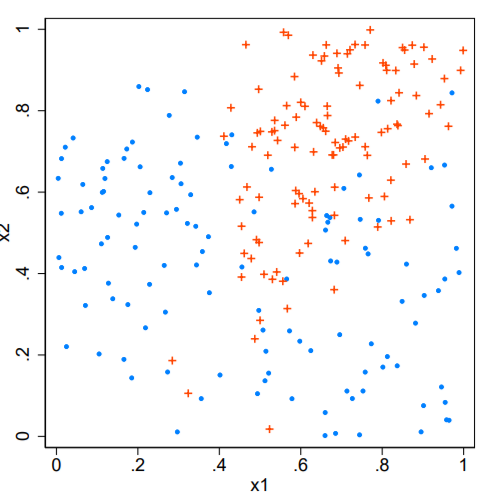
\includegraphics[width=\textwidth]{Classification with two classes.png}        
   % \caption{}
    \label{fig:my_label}
\end{figure}
\begin{itemize}
    \item To classify observations, a curve is drawn to delineate the classification boundary.
    \item  Since the two classes overlap, it's not possible perfectly separate the observations.
    \item It's possible to draw multiple boundary curves - resulting in more than 2 regions - and assigning multiple regions to the same outcome.
    \item In practice, observations from different classes are almost always overlapping on the observed features (here $x_1$ and $x_2$).
\end{itemize}

\begin{itemize}
    \item Classification tasks may involve more than two classes.
    \item Multiple curves are needed to separate them into regions.
    \item If classification were error-free in general, the problem would no longer be stochastic and not fit as well with our understanding of statistical learning.
\end{itemize}


\subsubsection{Supervised Learning: Regression}
\begin{itemize}
    \item Supervised learning with a known outcome that is continuous or is treated as continuous. 
    \item For most supervised statistical learning algorithms $f(x)$ is unknown and must be estimated from data.
    \item It is usually not possible to write down an equation for the estimated function $\widehat{f}(x)$ as the number of parameters is unknown. 
    \item Because of the lack of interpret ability we sometimes call such models \emph{Black Box Models}
    \item For more complicated relationships, we need a learning algorithm that accounts for: 
    \begin{itemize}
        \item Discontinuities
        \item Non-linearity
        \item Non-constant variance
    \end{itemize}
    \item Note: It's still possible but tedious to fit such data using separate straight lines for different x-regions.
\end{itemize}
\begin{figure}[!ht]
    \centering
    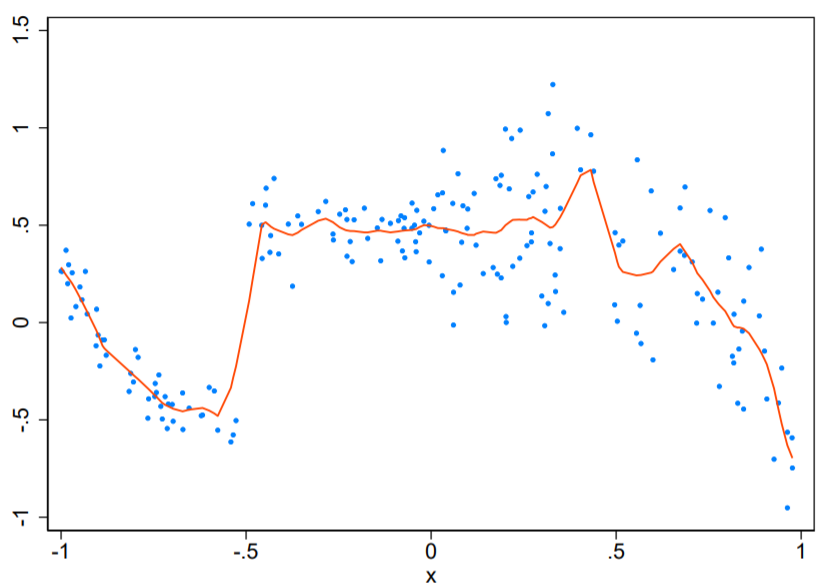
\includegraphics[width=\textwidth]{Regression with one x-variable.png}        
   % \caption{}
    \label{fig:my_label}
\end{figure}

\subsection{Unsupervised Learning/Clustering}

Identifying clusters of observations when group membership is 
unknown.

\begin{figure}[!ht]
    \centering
    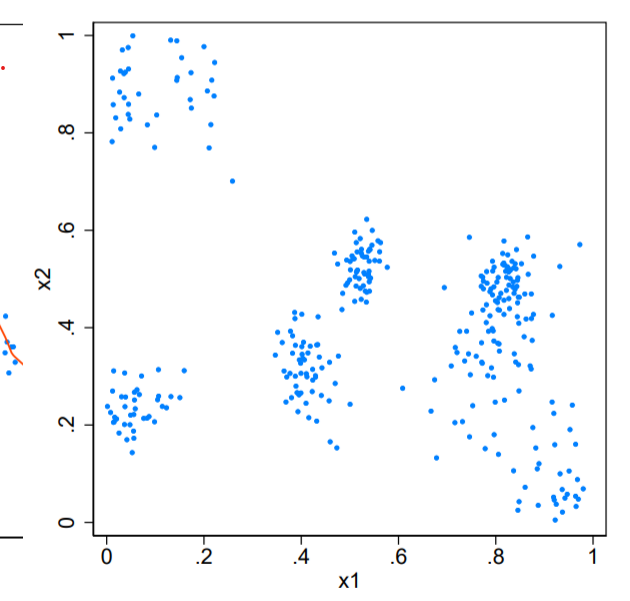
\includegraphics[width=\textwidth]{    Unsupervised Learning Finding clusters of observations.png}        
   % \caption{}
    \label{fig:my_label}
\end{figure}

\begin{itemize}
    \item Outcome is unknown.
    \item Most common task is clustering: Classifying observations into groups, but the training data don't contain class labels. (Number of groups may also be unknown)
    \item In practice, whether cluster assignments are correct or not is unknown (otherwise it would be supervised learning).
    \item However, we can explore the properties of cluster algorithms on simulated data sets where the correct cluster assignments are known. 
    \item Another unsupervised learning task is finding association rules: Finding interesting relationships between variables in a large data base.
\end{itemize}

\subsection{Interpretation versus Prediction}
\begin{itemize}
    \item Linear regression is not usually good at prediction.
    \item Although you can 
    \begin{itemize}
        \item log-transform an outcome $\by$ to achieve approximate linearity
        \item add interactions and quadratic terms
        \item diagnose multi-collinearity within x-variables
        \item use variable selection to remove unrelated x-variables (unrelated variables to y that just add noise)
    \end{itemize}
    more flexible statistical learning algorithms develop a suitable model automatically (subject to tuning) and they almost always beat linear regression in terms of prediction.
    \item The primary purpose of Gaussian linear regression is explanation: the linear model makes it possible to explain how an individual x-variable affects the outcome y: increasing $x_i$ by one unit is associated with an average increase in $y$ by $\beta_i$ units.
    \item The primary purpose of statistical learning is prediction.
    \item Statistical learning models (Black-box models) are free to be more complicated, capturing extra detail in the relationship between $x$ and $y$.
\end{itemize}
\subsection{The Bias-Variance Tradeoff}
Expected Mean Squared Error (MSE) = Variance + squared bias + irreducible error \\
where variance and squared bias are called reducible errors.
\begin{align*}
    E(y_0-\widehat{f}(x_0))^2 = Var(\widehat{f}(x_0)) + [Bias(\widehat{f}(x_0))] + Var(\eps)
\end{align*}
where $\widehat{f}$ is the estimated function and $x_0$ and $y_0$ are the test observation and true outcome.
\begin{itemize}
    \item A better estimator has smaller MSE.
    \item "Flexibility" of a fit refers to how local versus global a fit is.
    \item A highly flexible fit captures highly local behavior of the data but may also accidentally fit random noise.
    \item \textbf{As the learning algorithm learns increasingly local behavior, the bias is reduced.}
    \item \textbf{Learning about increasingly local behaviour must rely on fewer and fewer observations as observations farther away are no longer local $\implies$ resulting in higher variance}
    \item Highly local behaviour observed in any one data set may just be random noise. (\emph{Overfitting)}
    \item A less flexible fit is less prone to fit the noise. 
    \item A less local fit will also increase bias and will lead to \emph{underfitting}
    \item In the extreme, the model consists just of a constant $y=\Beta_0$ (A severely underfitting model)
\end{itemize}

\subsection{Bayes Error}
\begin{itemize}
    \item Test error: error in classifying new observations, is minimized if each test observation is assigned to the most probable class. 
    \item Bayes (Optimal) classifier: This classifier is optimal, on average. Note used in practice since, the true functional relationship between x-variables and the outcome $y$ is needed.
    \begin{align*}
        \underset{j}{max}P(Y=j|x)
    \end{align*}
    \item The Bayes error is the irreducible error. 
    \item However, we can assume a true function and evaluate the Bayes classifier on simulated data.
    \item Such simulations are useful for comparing any proposed new classifier with the Bayes classifier.
\end{itemize}

\subsubsection{Simulated Example in one dimension}
\begin{itemize}
    \item Consider a classification problem with two classes and a single continuous x-variable.
    \item x-values for each class are generated from a p.d.f. for that class.
    \item The figure below shows the known p.d.f for each class. 
    \item Given an x-value, we have to classify the observation(the x-value) into one of the two classes.
    \item Since we know the underlying distribution, we can compute the optimal Bayes decision boundary. 
    \item The Bayes error is minimized if we classify observations to whatever class has the larger probability.
    \item The figure below shows the p.d.f. crossing twice creating two decision boundaries. 
    \item Between the two boundaries, the observation is classified into the red class while the others are classified into the blue class.
\end{itemize}

\begin{figure}[!ht]
    \centering
    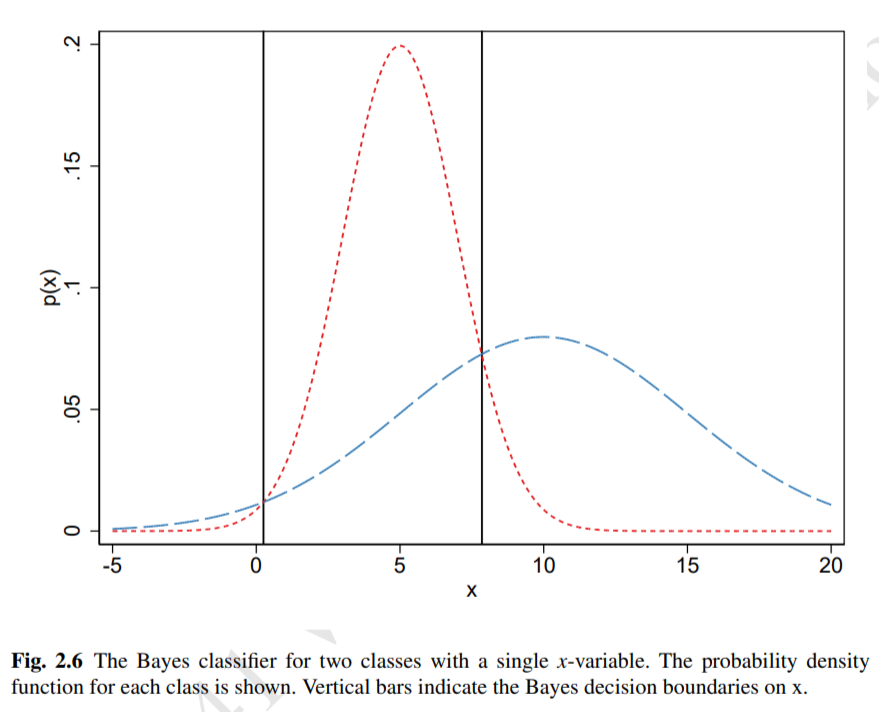
\includegraphics[width=\textwidth]{Bayes Classifier for two classes one x.png}        
   %\caption{}
   % \label{fig:my_label}
\end{figure}

\subsubsection{Simulated Example in two dimensions}
\begin{itemize}
    \item For each of two classes, the observations were generated from a weighted average of two bivariate Gaussian distributions (Mixture distribution).
    \item Here, the mixture distribution consist of 10 equally weighted bivariate Gaussian distributions. 
    \item Each of the 10 distributions is shown by red triangles for one class and blue triangles for the other class (All triangles with a black outline)
    \item Because the data is simulated, for any new observation we know which of the two classes has the higher probability. Therefore, we can compute the Bayes decision boundary.
    \item Since this Bayes decision boundary is optimal, we can later compare it with the decision boundary from another classifier trained on the data, but without knowledge of the underlying mixture distributions.
    \item Since the Bayes classification error is irreducible, the error rate achieved with the Bayes classifier is a lower bound on the error.
\end{itemize}


\begin{figure}[!ht]
    \centering
    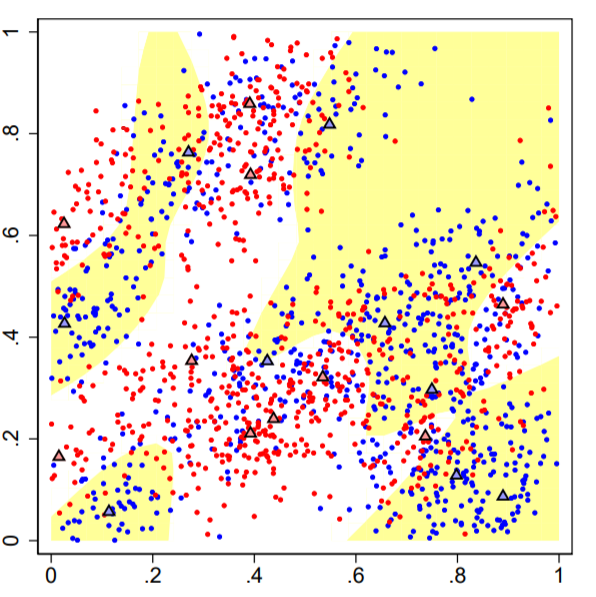
\includegraphics[width=\textwidth]{Bayes Classifier for two classes two x.png}        
   \caption{The Bayes decision boundary is the boundary between the white and yellow regions. The triangles give the means of the underlying mixture distributions.}
    \label{fig:my_label}
\end{figure}

\subsection{Summary}
\begin{itemize}
    \item The quest of better predictions leads us to look for more flexible models than linear regression.
    \item However, with increasing flexibility interpretation suffers.
    \item It is possible to develop methods to interpret more complex methods, but interpretation is inherently harder.
    \item Simulations can provide a baseline of how well a classifier can do relative to the Bayes error.
\end{itemize}



\newpage

\section{Logistic Regression}

\begin{itemize}
    \item Classifies observations into one of two classes with classification probability.
    \item Sometimes continuous variables are dichotomized: income can be dichotomized into "high income" or not.
    \item The two classes are coded as 0 and 1:
    \begin{align*}
        y_i = \begin{cases}
        1 & \text{if event i occurs} \\
        0 & \text{otherwise}
        \end{cases}
    \end{align*}
    \item In linear regression, the expected value E(y) is regressed on a linear function of x-variables.
    \item For logistic regression, denote the probability that the event occurs as $p$.
    \item Because there are only two outcomes, the expectation can be computed easily.
    $E(Y) = 1 \cdot p + 0 \cdot (1-p) = p$
    \item We would like to regress the expected value, p, on a linear function of x-variables.
    \item However, regressing $p$ directly on the x-variables is problematic: 
    \begin{itemize}
        \item The probability $p$ must take values between 0 and 1, but the linear function of the x-variables may take values outside of that range. 
    \end{itemize}
    \item Instead of regressing $p$ directly on the x-variables, regress a function of $p$ on the x-variables.
    \item A suitable function takes values from the real line ($-\infty, +\infty$) as input and gives values in the interval [0,1] as output.
    \item One function is the \emph{logit}:
    \begin{align*}
        \text{logit}(p) = \log \frac{p}{1-p}
    \end{align*}
    \item If $p$ = 0 or 1 the logit function is not defined, but that implies the event never occurs or always occurs
    \item Case 1: Only 1 x-variable
    \begin{align*}
        \text{logit}(p) = \log \frac{p}{1-p} = \beta_0 + \beta_1x
    \end{align*}
    \item Solving for $p$, we obtain the logistic function or \emph{expit} function:
    \begin{align*}
        p = \textsf{expit}(\beta_0 + \beta_1x) = \frac{e^{\beta_0 + \beta_1x}}{1 + e^{\beta_0 + \beta_1x}}
    \end{align*}
    \begin{itemize}
        \item The shape of this function - the probability as a function of x - is called "sigmoidal".
        \item Changing the intercept would result in shifting the curve to the right or left on the x-axis.
        \item Adding additional x-variables to logit(p) gives the full logistic regression model:
        \begin{align*}
            \log \frac{p}{1-p} = \beta_0 + \beta_1x_1 + \dotsb + \beta_px_p
        \end{align*}
        \item Because the equation is expressed in terms of expected values $E(Y) = p$ rather than Y itself, the logit equation above has no residual or error term.
        \item It is not deterministic, however: the uncertainty is represented through the probability p.
    \end{itemize}
\end{itemize}

\begin{figure}[!ht]
    \centering
    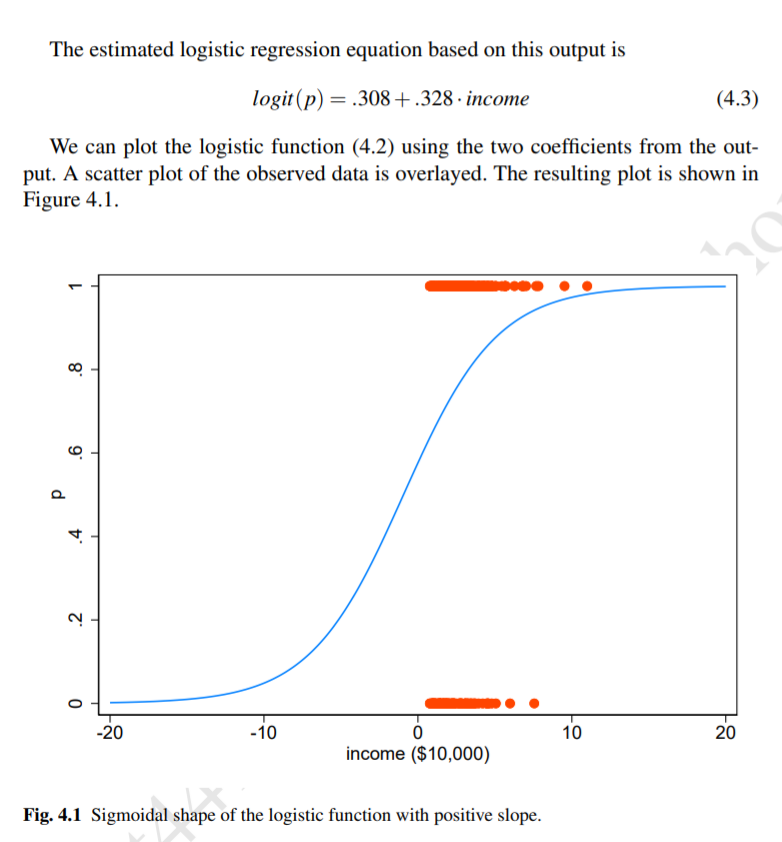
\includegraphics[width=\textwidth]{Sigmoidal shape of the logistic function with positive slope.png}        
   \caption{Sigmoidal shape of the logistic function with positive slope.}
    \label{fig:my_label}
\end{figure}


\begin{figure}[!ht]
    \centering
    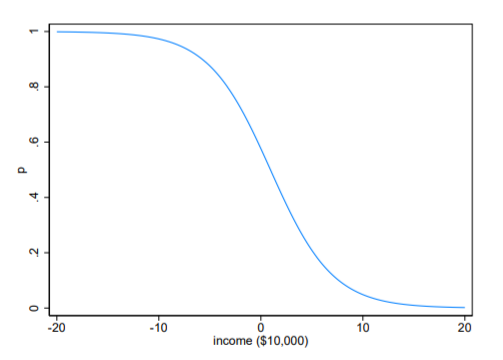
\includegraphics[width=\textwidth]{Sigmoidal shape of logistic function with negative slope.png}        
   \caption{Sigmoidal shape of the logistic function with negative slope.}
    \label{fig:my_label}
\end{figure}

\subsection{Prediction}
\begin{itemize}
    \item The goal of prediction is to classify an unseen observation into one of the two classes.
    \item The predicted probability can be computed using the expit:
    \begin{align*}
        p = \text{expit}(\beta_0 + \beta_1x_1 + \dotsb + \beta_px_p) = \frac{e^{\beta_0 + \beta_1x_1 + \dotsb + \beta_px_p}}{1 + e^{\beta_0 + \beta_1x_1 + \dotsb + \beta_px_p}}
    \end{align*}
    \item Then we can classify a new observation $i$ as
    \begin{align*}
        \widehat{y_i} = \begin{cases}
        1 & \text{if } p_i \leq t \\
        0 & \text{otherwise}
        \end{cases}
    \end{align*}
    where t is a threshold value.
    \item Most common threshold value is $t$ = 0.5 and this threshold corresponds to rounding the probability to either 0 or 1.
    \item Each threshold corresponds to a tradeoff between two types of errors:
    \begin{itemize}
        \item False negatives (Sensitivity)
        \item False positives (Specificity)
    \end{itemize}
    \item An ROC curve plots the tradeoff for a particular threshold between sensitivity and specificity
\end{itemize}

\subsection{Interpretation of the Coefficients}
\begin{itemize}
    \item Suppose the "Odds of winning are 3:2". The word \emph{odds} has a formal statistical definition:
    \begin{align*}
        \text{odds} \frac{p}{1-p}
    \end{align*}
    \item Then the odds are equal to 1.5. Solving for $p$, we obtain $p$ = 0.6
    \item The intercept $\beta_0$ can be interpreted as a \emph{log odds} in case all x-variables are 0.
    \begin{align*}
        \Log\frac{p}{1-p} = \beta_0
    \end{align*}

    \item The slope coefficients can be interpreted as so-called \emph{log odds ratios} (log OR), the log of the ratio of two odds.
    \item Consider the logistic regression with one x-variable. 
    \item To interpret the slope $\beta_1$ consider the same equation twice: once with $x$ for observation $j$ and one with $x$ increased by one unit for observation $i$:
    \begin{align*}
        \Log\frac{p_i}{1-p_i} &= \beta_0 + \beta_1(x_i + 1) \\
        \Log\frac{p_j}{1-p_j} &= \beta_0 + \beta_1x_j
    \end{align*}
    \item Taking differences gives
    \begin{align*}
         \Log\frac{p_i}{1-p_i} -  \Log\frac{p_j}{1-p_j} &= \beta_1(x+1) - \beta_1(x) = \beta_1 \\
         \beta_1 &= \Log\frac{\frac{p_i}{1-p_i}}{\frac{p_j}{1-p_j}} = \Log\frac{\text{odds}_i}{\text{odds}_j} \\
         \text{exp}(\beta_1) &= \frac{\text{odds}_i}{\text{odds}_j}
    \end{align*}
    \item So $\text{exp}(\beta_1)$ can be interpreted as the factor by which $\text{odds}_j$ increase:
    \begin{align*}
        {\text{odds}_j} \cdot \text{exp}(\beta_1) = \text{odds}_i
    \end{align*}
    \item For example, if $\beta_2 = 2$, increasing $x_2$ by 1 unit increase the odds of the event by a factor of exp(2) on average.
    \item If $x_2$ is an indicator variable with values 0 and 1, then turning the indicator variable on increases the odds of the event by a factor exp(2).
    \item The increase in odds is multiplicative, not additive. Such statements hold regardless of the values of other x-variables.
    \item A two-way interaction, $x_ij$, between two variables $x_i$ and $x_j$ is defined by multiplying the two variables with one another $x_ij = x_i \cdot x_j$. The factor that increases the odds depends on the level of a second variable.
\end{itemize}

\subsection{Estimation}

\begin{itemize}
    \item The coefficients are estimated by maximum likelihood.
    \item Assuming that the response is Bernoulli distributed, $Yi \sim Bernoulli(p_i)$, the likelihood for $n$ observations is:
    \begin{align*}
        L(\beta) = \prod_{i=1}^{n}([p_i(x_i;\beta)]^{y_i} \cdot [1-p_i(x_i;\beta)]^{1-y_i})
    \end{align*}
    where
    \begin{align*}
        p_i(x_i;\beta) =\frac{e^{x^t_i\beta}}{1+ e^{x^t_i\beta}} 
    \end{align*}
    where $\beta = (\beta_1,...,\beta_p)^T$ is the vector of coefficients and $x_i = (x_1,...,x_p)^T$ is the vector of observed values for observation i.
    \begin{itemize}
        \item The response, $y_i$ is a scalar
        \item For ease of notation we dropped $\beta_0$. A column of 1s as the last x-variable can be added which $\beta_p$ corresponds to.
    \end{itemize}
    \item Since the logarithm is a monotone function (non-increasing or non-decreasing), taking the logarithm on both sides does not affect the estimates of $\beta$. (The value of the maximum changes but not the location).
    \item The log likelihood is:
    \begin{align*}
        l(\beta) &= \sum^n_{i=1}\{{y_i} \cdot \log p_i(x_i;\beta) + {1-y_i} \cdot \log[1-p_i(x_i;\beta)]\} \\
        &=\sum^n_{i=1}\{y_i\beta^Tx_i - \}\\
    \end{align*}
\end{itemize}

\subsection{Summary}
\begin{itemize}
    \item Logistic regression is suitable for binary outcomes
    \item More flexible statistical learning models sometimes fail to beat it in terms of prediction, in particular for reasonably sized data sets in which most x-variables are indicator variables. 
    \item When number of variables exceeds the number of observations, logistic regression on the full set of variables will not run and more flexible learning algorithms or a regularized version of logistic regression or model selection is needed.
\end{itemize}

\newpage

\section{Chapter 3: Practical Aspects}
\subsection{Overfitting}
\begin{itemize}
    \item Fitting data so locally fit captures random noise
    \begin{figure}[ht]
    \centering
    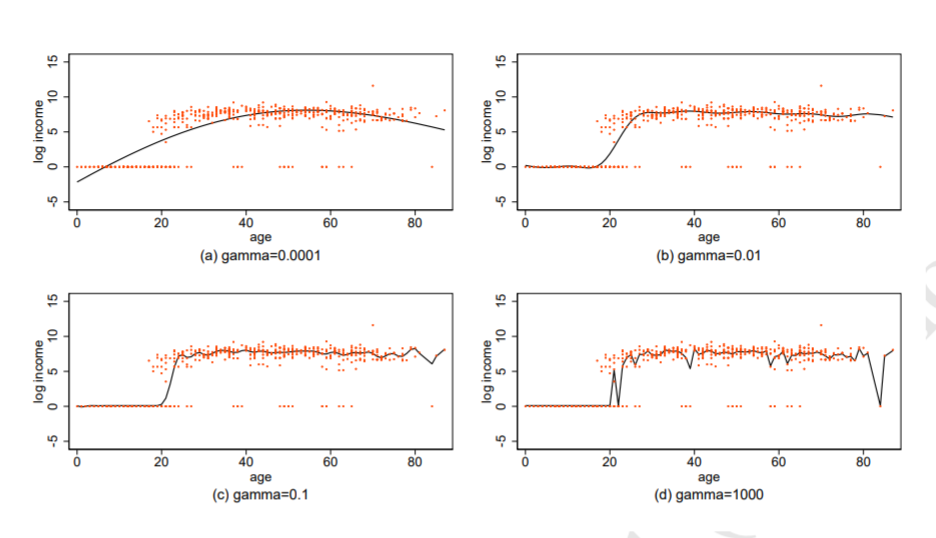
\includegraphics[width=\textwidth]{Fit of SVM.png}       
    \label{fig:my_label}
    \end{figure}
\item a is underfit, d is overfit, (b,c) are compromises (felxible without apparent overfitting).
\end{itemize}
\subsection{Training/Validation/Test data sets}
\begin{itemize}
    \item Typically, you will train your model not once but multiple times with different values for its parameters. (IE using multiple k values for k-nn)
    \item \textbf{Multiple comparison/Multiple Testing Problem}: Suppose we split the data into training data and 10 separate test data sets of equal size. Choosing the best of the 10 results would result in a problem.
    
    \item Split the data into 3 subsets:
    \begin{itemize}
        \item Training
        \item Validation: Used to choose the best model. This comes at the cost of having less data for training and validation. 
        \item Testing: Used to evaluate how well the best model performs. The test data must only be used once, after selecting the best model.
        \item Note: A two way split between training/testing can be idea if the sole purpose is to predict as well as you can. The role of the testing data in two-subset split and validation data in the three-subset split is the same. 
        \item Typical split = 60/2/
        0/20 train/validation/testing
    \end{itemize}
\end{itemize}
\subsection{Cross-validation}
\begin{itemize}
    \item Splits the data multiple times, each time using a different, non-overlapping validation data set, making it possible to validate on 100\% of the data or even increasing the training data size. 
    \item Primary focus is evaluation, not prediction.
\end{itemize}


\subsubsection{k-fold cross-validation}
Common values for k are 5 and 10.
\begin{lstlisting}
#Partition data in k random subsets of roughly equal size
for i=1 to k do
    subset[i] = validation data
    subset[j for j in range(k) if j != i] combined as training data
    Fit the model to the training data
    Evaluate the model on the validation data
end for

Two Options
1) Average the predictions over k evaluation results (Better at assessing variability, can average over the k estimates and compute a standard deviation) 
2) Refit a single model on the whole training data and predict the test data
\end{lstlisting}

\subsubsection{Leave-one-out (LOO) Cross-validation}
\begin{itemize}
    \item Fit a model on all but one observation and use the model to predict the single left-out observation.
    \item Repeat for all observations. 
    \item LOO is not good for small to moderate data sets. 
    \item Increasing the size of training data decreases the bias. 
    \item 10-fold validation trains on 90\% of the data. 
    \item LOO trains on almost 100\% of the data (Very high bias).
    \item A larger k also increases variance for estimating the test error as the overlap between training data sets is increasing. 
    \item LOO severely underestimates sample to sample variance in estimating the test error. 
\end{itemize}
\section{Evaluation Criteria for Assessment}
\subsection{Confusion Matrix}
    \begin{figure}[ht]
    \centering
    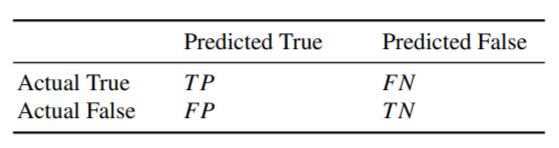
\includegraphics[width=\textwidth]{Confusion Matrix.png}       
    \label{fig:my_label}
    \end{figure}
\begin{itemize}
    \item \textbf{Accuracy}: $\frac{TP + TF}{N}$ 
    \item \textbf{Error Rate}: 1 - Accuracy
    \item \textbf{F-measure}: Range = 0 to 1. Higher values being better. 
    \begin{align*}
        F = \frac{2TP}{2TP + FP + FN}
    \end{align*}
    \item \textbf{Sensitivity}: \% of true positives correctly identified among the outcomes that are true. $$\frac{TP}{TP + FN}$$
    \item \textbf{Specificity}: \% of observations correctly classified among "no events" (True positive rate). 1 - Specificity = False positive rate.  $$\frac{TN}{TN + FP}$$
    Higher sensitivity and specificity is better. 
\end{itemize}
\subsection{Area under the ROC curve}
\begin{itemize}
    \item Sensitivity is plotted against the false positive rate (1 - sensitivity).
    \item Upper left corner of the graph represents high sensitivity with low false positive rate. 
    \item The 45 degree line is the reference (The value corresponding to random guessing).
    \item The orange triangle represents the threshold 0.5. This threshold corresponds to one particular tradeoff between sensitivity and specificity.  
\end{itemize}
\begin{figure}[ht]
    \centering
    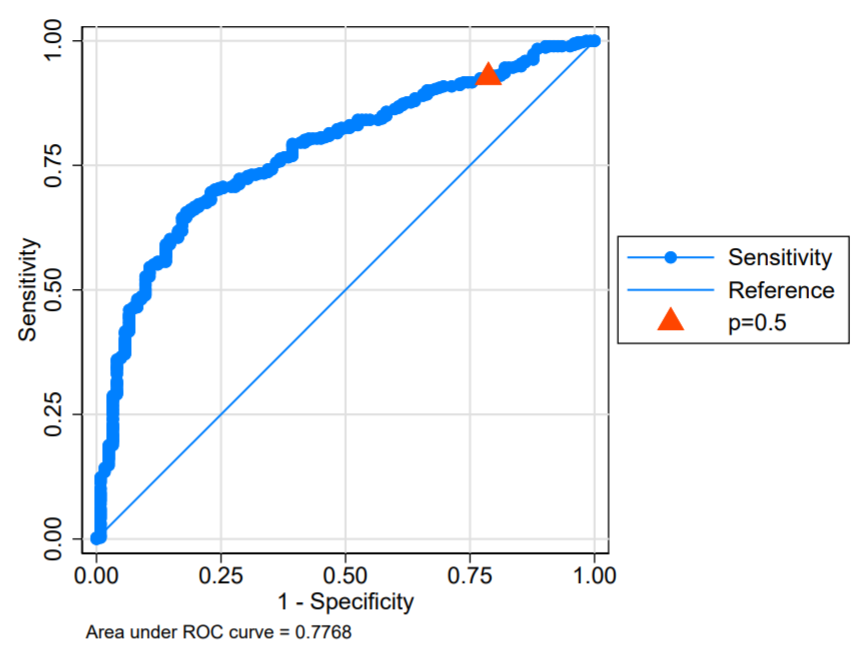
\includegraphics[width=\textwidth]{AUC.png}       
    \caption{The threshold 0.5 corresponds to 85\% sensitivity and a false positive rate (1- specificity) of 80\%}
\end{figure}

\subsection{Evaluation Criteria for Assessment}
\subsubsection{Criteria for Two-class outcomes}
\begin{itemize}
    \item \textbf{Cross-entropy}: Difference between classification and estimated probabilities.
    \begin{align}
        E = - \sum_{i=1}^n (y_i \log (\widehat{p_i}) + (1 - y_i)\log(1- \widehat{p_i}))
    \end{align}
    where n is the number of observations, $y_i \in \{0,1\}$ and $p_i = P(y_i = 1)$.
    \begin{itemize}
        \item Equation (1) is also the negative log-likelihood for a bernoulli distribution. 
        \item Maximizing log-likelihood is equivalent to minimizing the negative log-likelihood.
    \end{itemize}
    
    \item \textbf{Deviance}: A likelihood ratio test that compared a proposed model to the saturated model (The best possible model in which every observation is fitted exactly without error). 
    \begin{align*}
        D = 2(\text{log likelihood of saturated model - log likelihood of proposed model)}
    \end{align*}
    \begin{itemize}
        \item Since the log-likelihood of the saturated model is constant, minimizing deviance is equivalent to minimizing the negative log-likelihood of the proposed mode. 
        \item Specifically,m the deviance for the Bernoulli distribution - appropriate for outcomes with 2 classes is: 
        \begin{align}
            D = 2\sum_{i=1}^n (y_i \log (\frac{y_i}{\widehat{p_i}}) + (1 - y_i)\log(\frac{1 - y_i}{1 - \widehat{p_i}}))
        \end{align}
        where n is the number of observations and $y_i ~ \sim Bernoulli(p_i)$
    \end{itemize}
    Note: Minimizing (1) and maximizing (2) are equivalent.\\
    This criterion is also referred to as \emph{log loss}.
\end{itemize}

\subsubsection{Criteria for multi-class outcomes}
\begin{itemize}
    \item Classes that occur infrequently in multi-class outcomes are called \emph{rare classes}.
    \item \textbf{Accuracy with micro-averaging}: The average is computed over individual observations (Each observation has equal weight). 
    \item \textbf{Accuracy with macro-averaging}: When the distribution of classes is very uneven, it may make more sense to compute it as an average of ac curacies across all classes. 
    \textbf{Deviance}:
    \begin{align*}
        E = - \sum^n_{i=1}\sum^K{k=1} I(y_i = G_k)log(p_{ik})
    \end{align*}
\end{itemize}

\subsubsection{Criteria for Continuous Outcomes}
\begin{align*}
    RMSE  = \sqrt{\frac{1}{n}\sum^n_{i=1}(y_i - \widehat{f}(x_i))^2}
\end{align*}

\subsection{Regulating bias-variance tradeoff with tuning parameters}
\begin{itemize}
    \item More flexible fits exhibit more local behaviour. Too flexible results in random noise captured. 
    \item MSE cannot decrease to zero if there are duplicates. 
\end{itemize}

\subsection{One-hot encoding of categorical variables}
\begin{align*}
    E(y) &= \beta_0 + \beta_{\text{color}}x\\
    &=  \beta_0 + \beta_rI_{\text{red}} + \beta_yI_{\text{yellow}} + \beta_bI_{\text{blue}} \\
    &= \beta_0 + \beta_r({1 - I_\text{yellow} - I_\text{blue}}) + \beta_yI_{\text{yellow}} + \beta_bI_{\text{blue}}\\
    &= (\beta_0 + \beta_r) + (\beta_y-\beta_r)I_{\text{yellow}} + (\beta_b-\beta_r)I_{\text{blue}}
\end{align*}
Thus, baseline is the color red.

\subsection{Variable Scaling}
Statistical learning algorithms that are \emph{sensitive} to scaling: 
\begin{itemize}
    \item Distance-based algorithms (knn, SVM, gradient descent(neural networks)
    \item Penalized linear and logistic regression
\end{itemize}

Statistical learning algorithms that are \emph{insensitive} to scaling: 
\begin{itemize}
    \item Tree based algorithms (CART, gradient boosting, random forests)
    \item Algorithms that consider one variable at a time (Naive Bayes)
\end{itemize}


Two ways to scale:
\begin{enumerate}
    \item Standardize the variable to have mean 0 and variance of 1.
    \begin{align*}
        x_std = \frac{x - \barx}{\sigma}
    \end{align*}
    \item \emph{Standardization}: Indicator variables only take the values 0 and 1. Scale variables such that they have the same range, often [0,1]:
    \begin{align*}
        x_sc = \frac{x - min(x)}{max(x)-min(x)}
    \end{align*}
\end{enumerate}

\subsection{Reproducibility}
\begin{itemize}
    \item Program should be reproducible
    \item Set a random seed
    \item Then run with different/random seeds to test the variability of the result 
\end{itemize}


\section{Lasso and Friends}
When using generalized linear models, considering bias-variance tradeoff is helpful. We may be willing got tradeoff a little bias for a large reduction in variance. This may not lead to "right" coefficients but that doesn't matter if the goal is prediction. The usual estimation of regression coefficients does not address the bias-variance tradeoff. Regularized or penalized linear models include a penalty in the loss function that regulates this tradeoff as part of
the estimation.

\subsection{Regularized Linear Regression}
\begin{itemize}
    \item The vector $\beta = (\beta_0, \beta_1,...,\beta_p)^T$ is estimated using OLS estimator.
    \item OLS estimator is the minimum variance estimator among unbiased estimators in the class of linear models (Gauss-Markov theorem). 
    \item Regularized regression regulates the bias-variance tradeoff by introducing a criterion with a penalty(By reducing the coefficients that are badly estimated (ie. with low variance) to shrink faster than those that are well estimated (ie. low variance):
    \begin{align*}
        Criterion &= MSE + Penalty \\
        &= RSS/n + Penalty \\
        &= \sum^n_{i=1}(y_i - \beta^Tx_i)^2
    \end{align*}
    \item Dividing by n rather than by (n-df) ignores the (df) that are usually subtracted for unbiased estimation . For larger n, the effect of (df) is negligible. 
    \item All x-variables must be standardized to have mean 0 and variance 1 to avoid the solution for any particular penalty to depend on measurement units. 
    \item y-variable can also be standardized: when both x and y variables are standardized in linear regression, the intercept is 0. 
\end{itemize}

\subsubsection{Ridge Regression}


\begin{itemize}
    \item Linear regression with a \emph{Euclidean} or \emph{L2} penalty:
    \begin{align*}
    Criterion = \frac{RSS}{n} + \sum^p_{j=1}\beta^2_j
    \end{align*}
    \item Penalty is not applied to the intercept.
    \item Penalty favors smaller squared coefficients.
    \item To regulate how large the penalty should be relative to RSS/n: introduce a tuning parameter $\lambda > 0$
    \begin{align*}
    Criterion = \frac{RSS}{n} + \lambda\sum^p_{j=1}\beta^2_j
    \end{align*}
    \item $\lambda$ usually estimated via 10-fold cross validation. For each hold-out fold, the MSE is computed. $\lambda$ is then chosen to minimize the average MSE on the 10 hold-out folds. 
    \item In ridge regression, coefficients will not be exactly 0, so it is not a good tool for variable selection.
    \item Mean prediction squared error = average of MSE computed on hold out samples. 
    \item Choosing a slightly larger $\lambda$ not more than 1 standard error from the minimum has the advantage that fewer variables are chosen. (The resulting model becomes more interpretable)
\end{itemize}

\subsubsection{Lasso}
\begin{itemize}
    \item If we don't want to penalize large coefficients as strongly, penalize the \emph{absolute value}:
    \begin{align*}
        Criterion = \frac{RSS}{n} + \lambda\sum^p_{j=1}|\beta_j|
    \end{align*}
    \item Since coefficients shrink faster than the L2 penalty under the L1 penalty, the lasso is a better tool for variable selection. 
    \item Usually, lasso performs better than ridge regression and when there are a lot of irrelevant variables in the data and only worse when the variables are highly correlated.
    \item When x-variables are correlated, the lasso tends to select one of them and discard the remainder. 
    \item When $p:parameters > n$ the lasso selects at most n variables.
\end{itemize}

\subsection{Elastic Net}
\begin{itemize}
    \item A compromise between ridge regression and the lasso. 
     \begin{align*}
        Criterion = \frac{RSS}{n} + \lambda(\alpha\sum^p_{j=1}|\beta_j| + \frac{1 - \alpha}{2}\sum^p_{j=1}\beta_j^2)
    \end{align*}
    where $0 \leq \alpha \leq 1$ and $\lambda > 0$.
    \item Elastic net encourages highly correlated variables to either stay in the model as a group or to leave the model as a group. 
    \item Preferable to lasso in the case where p ($\#$ parameters) is much greater than n (observations). 
\end{itemize}

\begin{itemize}
    \item For linear regression, the goal was to minimize the penalized RSS criterion.
    \item Now the goal is to maximize the penalized log likelihood criterion.
    \item for L2 penalty, maximize:
    \begin{align*}
    Criterion = loglikelihood - \lambda\sum^p_{j=1}\beta^2_j
    \end{align*}
    \item For L1 penalty, maximize:
    \begin{align*}
        Criterion = loglikelihood - \lambda\sum^p_{j=1}|\beta_j|
    \end{align*}
    \item Because the criterion is maximized, the penalty is subtracted rather than added like before. 
\end{itemize}

\subsection{Inference}
\begin{itemize}
    \item Regularized regression works well for prediction or estimating coefficients. 
    \item If we run an OLS regression with the set of variables selected by a lasso, the standard errors will be incorrect: The OLS regression does
    not reflect the uncertainty in selecting variables; it assumes you always wanted to use that specific subset of variables. 
    \item Solution: partition x-variables into two sets. 
    \begin{itemize}
        \item Covariates: key x-variables.
        \item Control variables: larger set of variables of which only a subset is though to be part of the true model.
    \end{itemize}
    
    \item \textbf{Double Selection}:
    \begin{enumerate}
        \item Run lasso of y on the control variables
        \item Run lasso of each key x-variable on the control variables
        \item Identify the union of all x-variables in any of the lasso regressions
        \item Regress y on the key x-variables and the union of selected control variables
    \end{enumerate}
\end{itemize}

\subsection{Imputation of Missing values}
\begin{itemize}
    \item Most common strategy to address missing values is to impute them: predict a suitable value that is consistent with other covariates.
\end{itemize}

Standard Dev. (SD) = $\frac{1}{n-1}\sum^n_{i-1}$ \\
Standard error = $\frac{SD}{\sqrt{n}}$

\newpage
\section{Working with Text Data}
\subsection{Turning Text into Variables}
\subsubsection{Text as a bag-of-words}
\begin{itemize}
    \item Give each word a variable = its occurrences ($t_cat = 3$)
    \item n\_token = total \# of words
    \item Ignores word order
\end{itemize}

\subsubsection{Stopwords}
\begin{itemize}
    \item Stopwords: the, a, is, to, that, etc.
    \item Knowing how often stopwords occur in a text is not helpful in classifying texts.
    \item Removing stopwords indiscriminately is not always a great idea.
\end{itemize}

\subsubsection{Stemming and Lemmatization}
\begin{itemize}
    \item The words "chases", "chased", and "chasing" are various inflections of the same word. 
    \begin{itemize}
        \item This group of inflected words will be represented by its canonical representative "chase". 
    \end{itemize}
    \item \textbf{Lemming}: Substituting an inflected word with its \emph{lemma}/canonical representation. 
    \begin{itemize}
        \item Usually leads to better predictive performance. 
    \end{itemize}
    \item \textbf{Stemming}: Applying a set of deletion and substitution rules to a word to identify the word stem. 
        \begin{itemize}
            \item Ex: "Chase" can be obtained from "Chased".
            \item Stemming doesn't always find a word's lemma. (Ex: go and went have the same lemma without sharing letters. Was, am , be, I'm have the same lemma.)
            \item Usually, \emph{Understem} or light stemming leads to better results
        \end{itemize}
\end{itemize}

\subsubsection{n-gram variables}
\begin{itemize}
    \item Bigrams: Variable for two-word sequence. (Ex: "Nigerian Prince" should be categorized as SPAM)
    \item n-gram: Variable containing "n" words.  
    \item Introducing higher order n-grams partially recovers word order. 
    \item \textbf{Threshold}: 
    \begin{itemize}
        \item Minimum number of texts in which the word has to occur before a variable is created.
        \item n-grams that occur only a few times across all text may not be helpful for prediction and can be discarded.
        \item Be wary of setting threshold too high(informative variables may be discarded).
        \item \textbf{Typical threshold}: 5
    \end{itemize}  
\end{itemize}
\subsubsection{Normalization}
\begin{itemize}
    \item Normalize words to a canonical version of the word
    \item Ex: all words encoded in lower-case (Cat = cat).
    \item Can be tricky: US (United States) != us
\end{itemize}

\subsubsection{Rescaling counts using TF-IDF}

\begin{itemize}
    \item \textbf{Document(D)}: text of one observation. 
    \item \textbf{Term}: "word".
    \item \textbf{Term frequency (TF)}: Dampens effect of additional words\\
    $$TF = \begin{cases}
        1 + log(f_{t,d}), & \text{ if } f_{t,d} > 0 \\
        0, & \text{otherwise}\\
    \end{cases} $$
    where $f_{t,d}$ is the number of times word t appears in document d. \item \textbf{Inverse document frequency(IDF)}: Some frequently used words may not be useful in discriminating among the texts. 
    \begin{align*}
        IDF = log(N/N_t)
    \end{align*}
    where N is the \# of documents, and $N_t$ is the number of documents containing the term t at least once. 
    \item TF-IDF: There are several minor variations of how to define this. 
    \begin{align}
        TF - IDF = TF \cdot IDF
    \end{align}
\end{itemize}

\subsubsection{Misspelled Words}
\begin{itemize}
    \item Look up all words in a dictionary and flag misspelled words. 
    \item Correct the words by computing the edit or Levenshtein Distance. 
    \textbf{Edit distance}: \# edits required to turn misspelled word into correctly spelled word. 
    \begin{itemize}
        \item Operations: add/remove/substitute char
        \item Ties solved by using the more common word. 
        \item Reduce computation: Limit search space to words with the same first letter. 
    \end{itemize}
\end{itemize}

\subsection{Why Linear and logistic regression does not work well for text}
\begin{itemize}
    \item \# of n-grams are typically large. $p >> n$
    \item Linear and logistic regression will fail when there are more parameters than observations. 
    \item Because each document only contains a limited number of words, most values of n-grams are 0. 
    \item This induces a high degree of collinearity among variables. 
\end{itemize}
\subsection{Summary}
Note: Indicator variables usually work better for short texts compared to a frequency count. 

\newpage
\section{Nearest Neighbors}

\subsection{k-Nearest Neighbors}
\begin{itemize}
    \item Suppose $x_0$ is a new observation to be classified.
    \item Optimal Bayes decision rule assigns the class j with highest probability:
    \begin{align*}
        \argmax_j P(Y=j|X=x_0)
    \end{align*}
    \item Unfortunately these probabilities are unknown. 
    \item k-nn estimates these probabilities locally. 
    \item Find the nearest k observations in the training data and define probabilities for each class
    \begin{align*}
        P(Y=k|X=x_0)=k_i/k
    \end{align*}
    where $k_i$ is the number of the k nearest neighbors from class i and k = $\sum^g_{i=1}k_i$.
    \item Example for k = 2:
    \begin{figure}[ht]
    \centering
     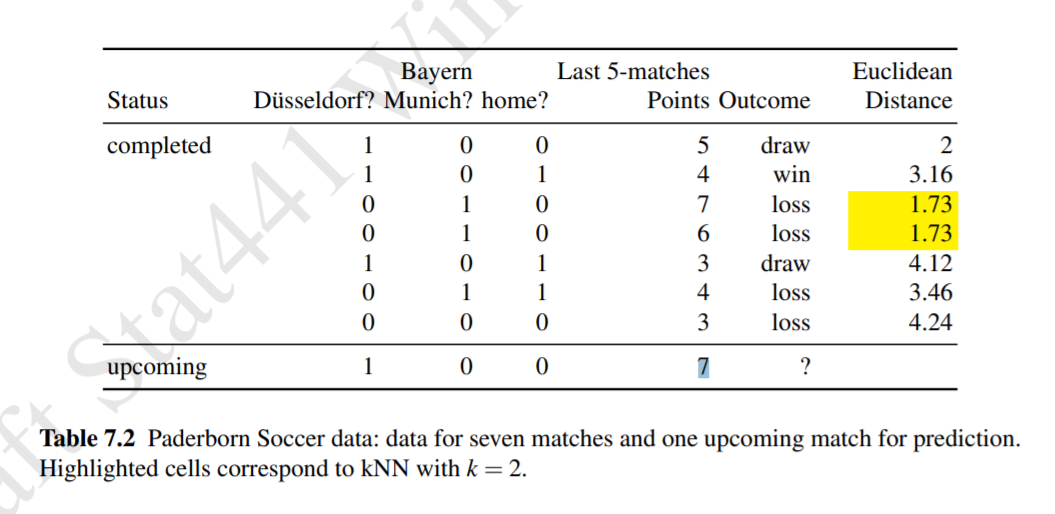
\includegraphics[width=1.0\textwidth]{2-nn-ex.png}
    \end{figure}
    \begin{align*}
        \text{P(Y=win$|$upcoming match)} = 0/2 = 0 \\
        \text{P(Y=draw$|$upcoming match)} = 0/2 = 0 \\ 
        \text{P(Y=loss$|$upcoming match)} = 2/2 = 0 
    \end{align*}
    based on the the two closest observations determined by euclidean distance.
    
    \item Class probabilities can also be computed as the posterior probability of classification using Bayes theorem:
    \begin{align*}
        P(Y=j|X=x_0) &= \frac{P(X=x_0,Y=j)}{P(X=x_0)} \\
        &= \frac{P(X=x_0|Y=j) \cdot P(Y=j)}{\sum^G_{i=1} [P(X=x_0|Y=i) \cdot P(Y=i)]}\\
        &= \frac{q_j k_j}{n_j} / \sum^G_{i=1}\frac{q_i k_i}{n_i}
    \end{align*}
    where G is the number of classes(groups), \\
    $q_j$ = P(Y=j) is the prior probability of class j, \\
    $k_j$ is the number of k nearest neighbors from class j, \\
    $n_j$ is the sample size of class j. 
\end{itemize}

\subsubsection{Prediction}
\begin{itemize}
    \item Predicted class = majority vote of the $k$ local observations. 
    \item If data contains exactly two classes, it is often better to choose an odd number to avoid ties. 
    \item If tie:
    \begin{itemize}
        \item Break ties at random.
        \item Increase $k$ until tie is broken.
        \item Use single nearest neighbor(1-NN) as tie breaker, there may however be more than one single closest observation resulting in another tie. 
    \end{itemize}
    \item For knn regression, the predicted value is the average of the response of the k nearest neighbors. 
    \item kNN is more often used for classification than in regression.
\end{itemize}

\subsubsection{Distance and Similarity}
Euclidian distance is often used in k-nn. Sometimes it is more convenient to specify a similarity measure instead of a distance measure. 
\begin{itemize}
    \item \textbf{Jacard Similarity Measure}: Can be used when all features are binary. Proportion of matches where the true negatives are excluded from denominator. 
    \begin{align*}
        S_{Jaccard}(ij) = \frac{TP}{TP + FN + FP}
    \end{align*}
     where $S_{Jaccard}(ij)$ is the similarity between two observations i and j. 
    \item \textbf{Euclidian Distance}: Works better for prediction when standardized.
    \begin{align*}
        d(x,j) = \sqrt{\sum^n_{i=1}(x_i - j_i)^2}
    \end{align*}
    \item \textbf{Cosine($x_0$,x) Similarity Measure}: Traditionally used in information retrieval (Ex: searching the web). Also called angular similarity because the cosine is a monotone decreasing function of the angle between two vectors.  
    
    \item Similarity to Distance conversion: Smallest distance = greatest similarity
    \begin{align*}
        d_1(ij) &= \sqrt{s(ii) + (sjj) - 2s(ij)} \\
        d_2(ij) &= 1 - s(ij) \\
    \end{align*}
    where s(ij) is the similarity between i and j.
\end{itemize}

\subsection{Properties of kNN}
\subsubsection{kNN accommodates nonlinear behavior}
kNN is highly flexible and approximates the Bayes classifier. The $k$ regulates the bias-variance tradeoff. 
\begin{itemize}
    \item Comparison of k-nn to logistic regression.
\end{itemize}
    \begin{figure}[ht]
    \centering
    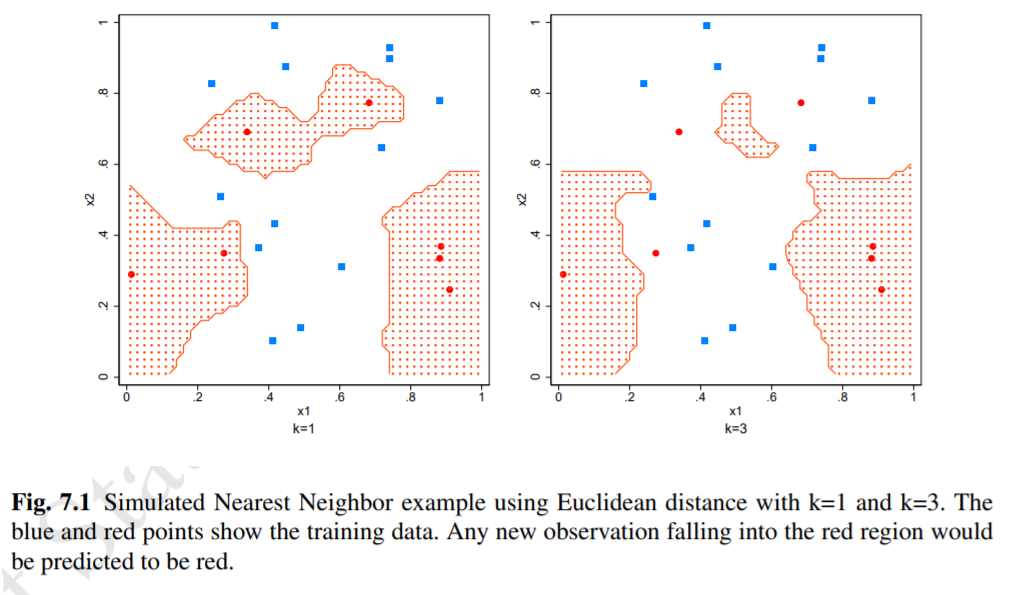
\includegraphics[width=\textwidth]{knn-1-3.png}       
    \label{fig:my_label}
    \end{figure}
    \begin{figure}[ht]
    \centering
    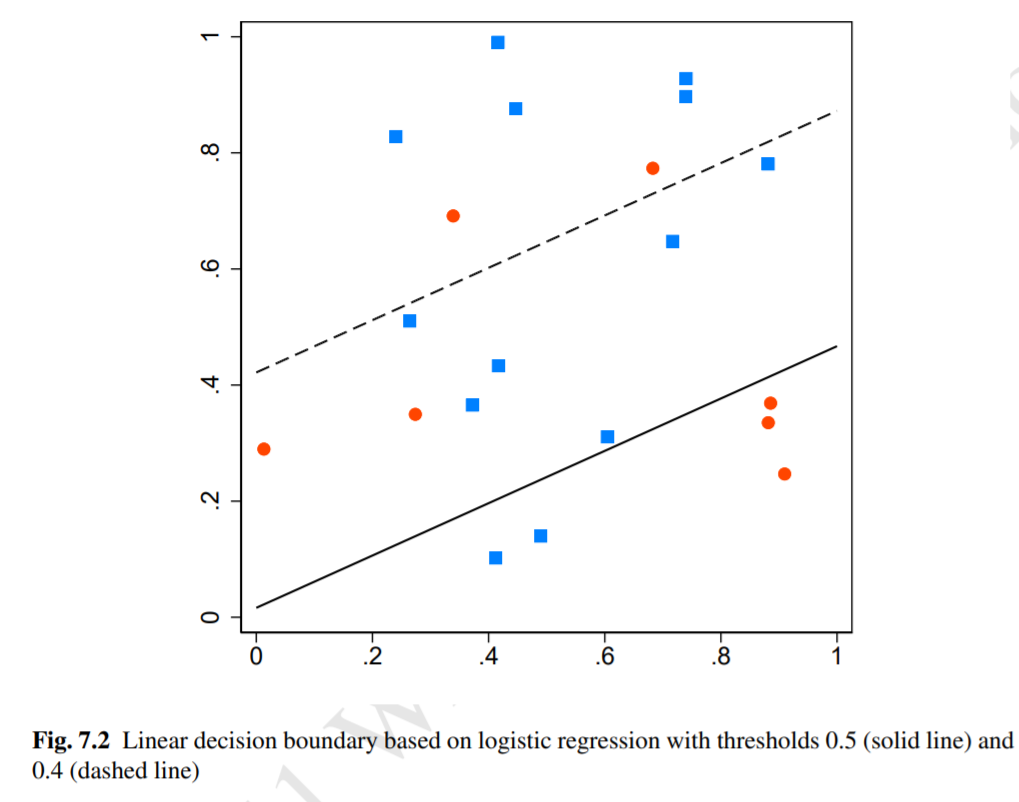
\includegraphics[width=\textwidth]{log-reg.png}       
    \label{fig:my_label}
    \end{figure}
\newpage
\subsubsection{kNN approximates the Bayes classifier}
\begin{itemize}
    \item The Bayes classifier assigns the class $j$ for which P(Y=j$|$X=$x_0$) is largest.
    \item However, this conditional can only be calculated when the underlying true model is known.
    \item P(Y=j$|$X=$x_0$) = $k_i/k$ attempts to approximate the conditional probability for a given class with a fraction of observations in a local neighborhood of k observations that correspond to that class. 
\end{itemize}

\subsubsection{k regulate  the Bias-Variance tradeoff}
\begin{itemize}
    \item Bias: Modelling $x_0$ as a function of only a few data points allowing for high flexibility (utilizing features of the closest data points but not the ones farther apart)
    \item For the choice of k = 1, the algorithm is highly local and has low bias. However, the prediction is only based on a single observation so the variance of the estimate is high.
    \item Increasing $k$ also increases the average distance of the $k$ training obs to $x_o$: so bias increases.
    \item The test error initially decreases because the reduction in variance is larger than the increase in bias as $k$ increases. At some point this reverses leading to a U-shape for the test error. 
    \item The fact that training is not strictly monotonically increasing and the U-shape of the test error is also not a perfect "U" are a reminder that the curves are estimated and the estimates are subject to variability.
    \item There is no point in trying to decide whether k should be 49, 50, 51 based on a single test error curve when a different random split into training and test data might show a minimum at k = 40 or k = 30.
    \begin{figure}[!ht]
    \centering
    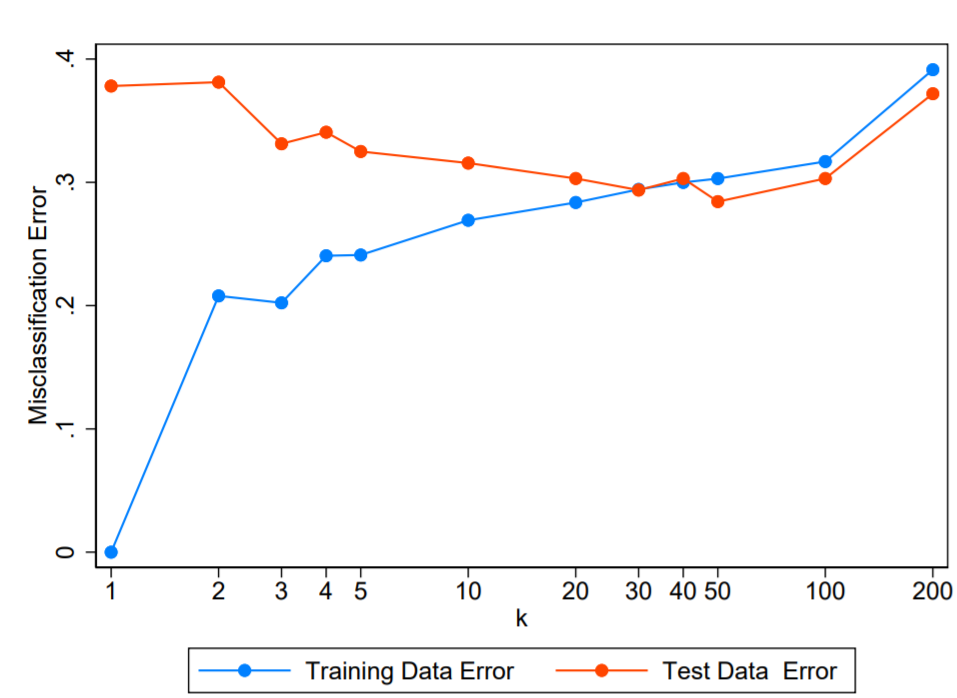
\includegraphics[width=\textwidth]{knn-error.png}       
    \label{fig:my_label}
\end{figure}
\end{itemize}

\subsubsection{kNN is sensitive to scaling}
\begin{itemize}
    \item To avoid some that some variables dominate determining the nearest neighbors, one option is to standardize/rescale variables. 
    \item Mahalonobis transformation: 
\end{itemize}

\subsubsection{kNN is slow and memory hungry}
\begin{itemize}
    \item For one test observation, the time to find the nearest neighbor is $O(n_{train} \cdot p)$ where $n_{train}$ is the number of training observations and p is the number of variables.
    \item In comparison, logistic regression has a time complexity of $O(p)$ for classification. 
    \item Training data needs to be stored which makes kNN memory intensive.
    \item Prediction based on linear regression only need to store $p$ coefficients.
    \item nn-classifiers are particularly easy to cross-validate with the leave-one-out technique. Since kNN doesn't require a model but simply looks up the nearest neighbors, LOO only needs to exclude the current observation.   
\end{itemize}

\subsubsection{Grid search for k and distance metrics}
\begin{itemize}
    \item 
\end{itemize}

\subsubsection{Summary}
\begin{itemize}
    \item kNN accommodates highly local behavior. 
    \item Works well when decision boundary is highly irregular and training data are sufficiently large.
    \item Not useful for learning how x-variables relate to outcomes.
\end{itemize}


\newpage
\section{Naive Bayes Classifier}

\subsection{Naive Bayes}
\begin{itemize}

    \item Using Bayes theorem to calculate the probability of an observation belonging to a class k:
    \begin{align*}
        P(Y=k|X=x) = \frac{\pi_kf_k(x)}{\sum^K_{l=1}\pi_lf_l(x)}
    \end{align*}
    where $f_k(x) = P(X=x|Y=k), x = (x_1,...,x_p)^T$ is the density conditional on class k and $\pi_k$ is the prior probability of class k.
    \item Now assume $x_j= 1,...,p$ are independent. This gives:
    \begin{align*}
        f_k(x)\prod^p_{j=1}f_{kj}(x_j)
    \end{align*}
    where p is the \# of x-variables and $f_{kj}(x_j) = P(X_j = x_j|Y=k)$ refers to the density of $x_j$ given Y = k.
    \item Since the denominator does not depend on k, to find the class that maximizes the posterior probability, we can ignore it giving:
    \begin{align*}
        P(Y=k, X=x) \propto \pi_k\prod^p_{j=1}f_{kj}(x_j)
    \end{align*}
    \item We predict the class k that maximizes the posterior probability:
    \begin{align*}
        \widehat{y} = \argmax_k\left(\pi_k\prod^p_{j=1}f_{kj}(x_j)\right)
    \end{align*}
    \item When there are too many x-variables, multiplying many small probabilities may result in a numerical "underflow". To avoid treating such probabilities as 0, use natural log. Since it is a monotone function, taking the log does not change which class k gives the maximum posterior probability. 
    \begin{align*}
        \widehat{y} = \argmax_k\left(\log(\pi_k) + \sum^p_{j=1}log[f_{kj}(x_j)]\right)
    \end{align*}
\end{itemize}

\subsubsection{Estimation}
\begin{itemize}
    \item \textbf{Prior probability}: $$\pi_k = \frac{n_k}{n}$$
    \item \textbf{Density} of \emph{Multinomial Naive Bayes}: When all x-variables are categorical.   $$f_{kj}(x) = P(X_j=x|Y=k) = \frac{n_{kj}}{n_k}$$ 
    \item \textbf{Density} of \emph{Gaussian Naive Bayes}: If at least one x-variable is a continuous variable:
    \begin{align*}
        f_{kj}(x_j) = \frac{1}{\sqrt{2\pi\sigma^2_{jk}}}exp\left[-\frac{1}{2}\left(\frac{x_j-\mu_{jk}}{\sigma_{jk}}\right)^2\right]
    \end{align*}
    where the means $\mu_{kj}$ and variances $\sigma_{jk}$ are estimated from the data. 
    \item Sometimes continuous variables are binned into categorical variables. (Income binned into low high). Thus, Gaussian Naive Bayes is not as common as multinomial Naive Bayes.
\end{itemize}

\subsection{Smoothing}
If one of the x-values did not occur for a given class k, the corresponding probability will be 0. Thus, the conditional probability of class k, P(Y=k, X=x) is 0 also. This causes a numerical problem when taking the log. Smoothing solves this problem by "shrinking" probability estimates away from the extremes avoiding probabilities of 0 and 1 altogether.

\subsubsection{LaPlace Smoothing and a generalization}
\begin{itemize}
    \item For a given x-variable, LaPlace smoothing adds one observation to each category:
    \begin{align*}
        P(X_j = x_j |Y=k) = \frac{n_{kj} + 1}{n_k + d_j}
    \end{align*}
    where $d_j$ is the \# of categories of the corresponding x-variable.
    \item Instead of adding just one observation, we can add an arbitrary number of observations, L (L does not have to be an integer):
     \begin{align*}
        P(X_j = x_j |Y=k) = \frac{n_{kj} + L}{n_k + L \cdot d_j}
    \end{align*}
    \item As L increases:
    \begin{align*}
        P(X_j = x_j |Y=k) \rightarrow 1/d_j
    \end{align*}
    
\end{itemize}

\subsubsection{The m-estimator}
\begin{itemize}
    \item m-estimator:
    \begin{align*}
        P(X_j = x_j |Y=k) = \frac{n_{kj} + m \cdot p_j}{n_k + m}
    \end{align*}
    where $p_j$, j = 1,...,$d_j$ is the prior probability of class $x_j$.
    \item Assuming a uniform prior, all outcomes are equally likely, we estimate $p_j$ = 1/$d_j$
    \item We can then think of m-estimator as adding m virtual observations, of which $m \cdot p_j$ fall into each class. 
    \item m is a tuning parameter analogous to L in the generalized LaPlace estimator. 
    \item For very large m
    \begin{align*}
        P(X_j = x_j |Y=k) \rightarrow p_j
    \end{align*}
    For the uniform prior, this has the same limit as that of the generalized LaPlace estimator.
\end{itemize}

\subsection{Summary and Remarks}
\begin{itemize}
    \item Naive Bayes Classification is easily scalable because the condition independence assumption allows estimating one variable at a time.
    \item For the same reason, Naive Bayes does not tend to need a lot of training data.
    \item Naive Bayes does good in prediction despite its wrong assumption of conditional independence. 
    \item Although the individual class density estimates may be biased, this bias might not hurt the posterior probabilities as much, especially near decision regions. 
    \item The problem may be able to withstand considerable bias for the savings in variance such a "Naive" assumption earns. 
    \item Naive Bayes Classification may not always give accurate estimates of probabilities. However, classification is fairly robust to inaccuracies in the probabilities because classification only depends on identifying which class has the \emph{largest} probability. 
\end{itemize}

\end{document}
